\documentclass[../main.tex]{subfiles}
 
\begin{document}

\section{Összefoglalás: Elkészült eszköz értékelése és költségterv számolása //TODO}
    \subsection{Az elkészült eszköz értékelése}
        Összesen 5 eszközhöz elegendő alkatrészt rendeltem meg, amelyekből 3 kész LED sor vezérlő került sikeresen elkészítésre. Kettő javított verziójú NYÁK-kal és egy pedig az eredetileg elkészített NYÁK-kal működik. Mind a három egység stabil, üzembiztos viselkedést mutat. Az egyik egység az otthoni teraszunkra (\ref{fig:pic_terasz}. ábra), a másik a kollégiumi szobába került felszerelésre. A harmadik egység tartaléként működik. A eszköz tesztelve lett akkumulátorrol is, egy Halloween-i jelmez kellékeként. Három cellás (12V-os), 2200mAh-s LiPo (Lithium Polimer) akkumulátorról üzemeltetve 5 órán keresztül működött. 
    
        \begin{figure}[h!]
            \centering
                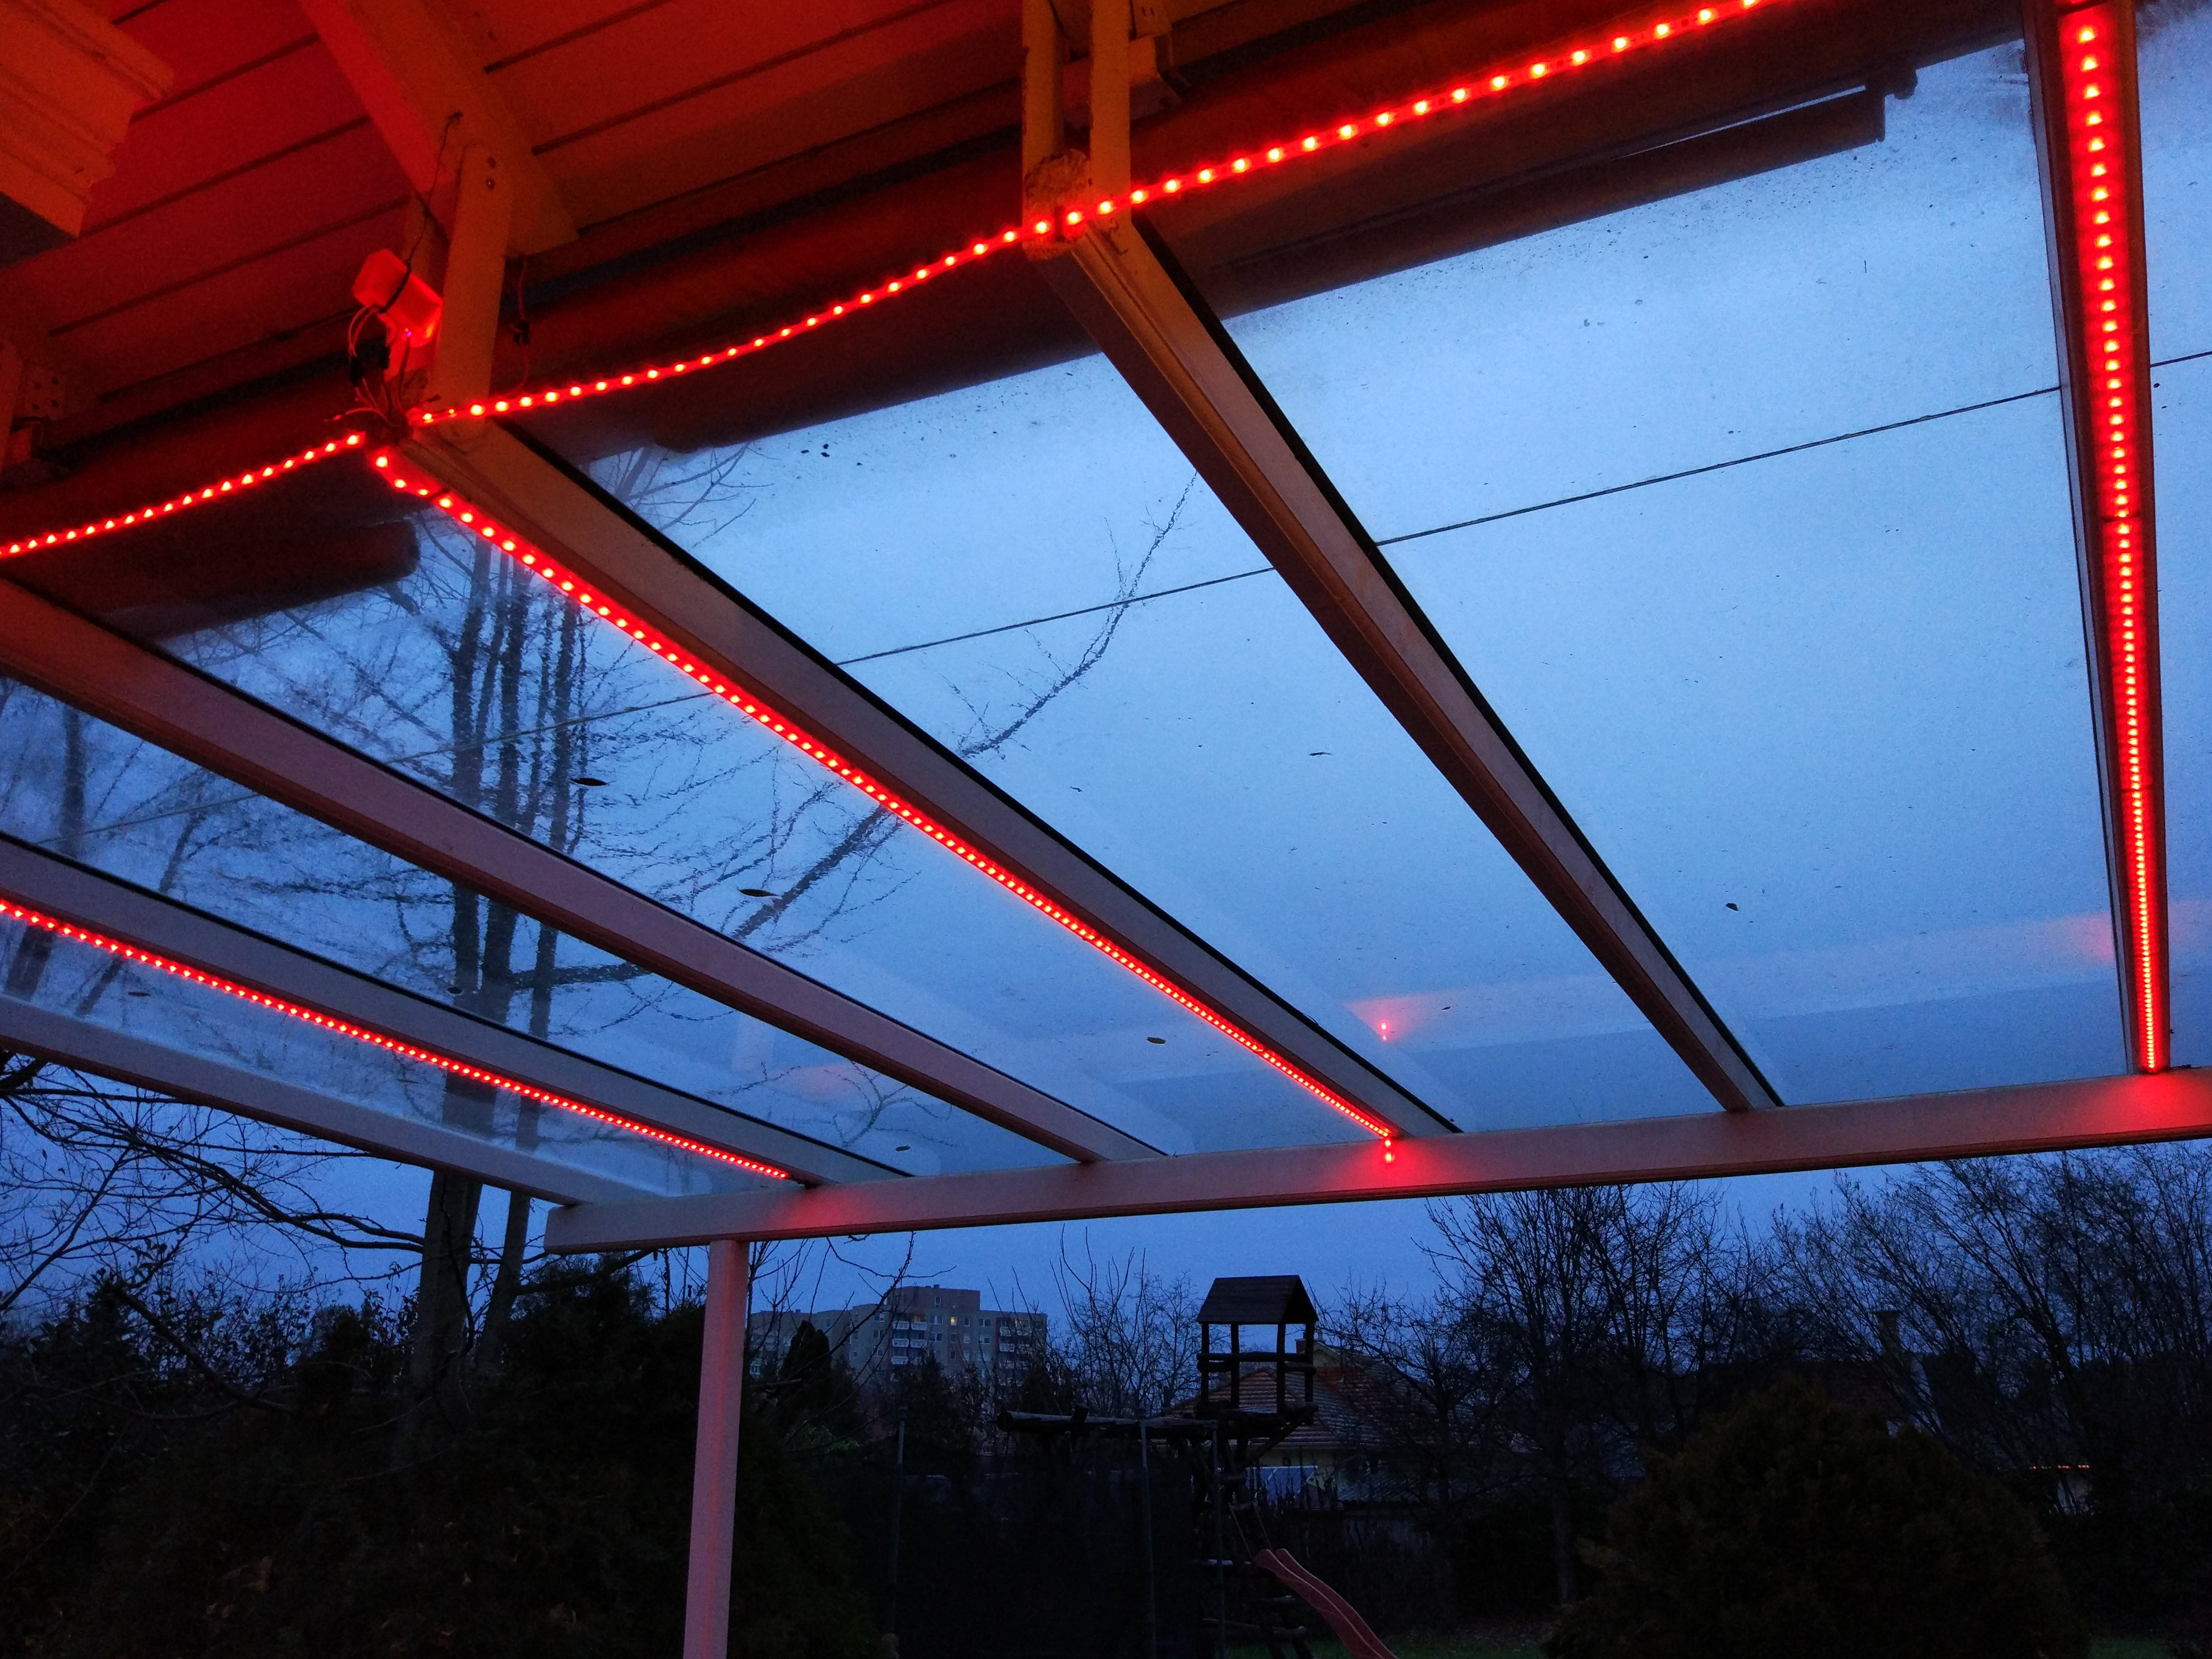
\includegraphics[height=3.8cm]{resources/alk_res/1_red}
                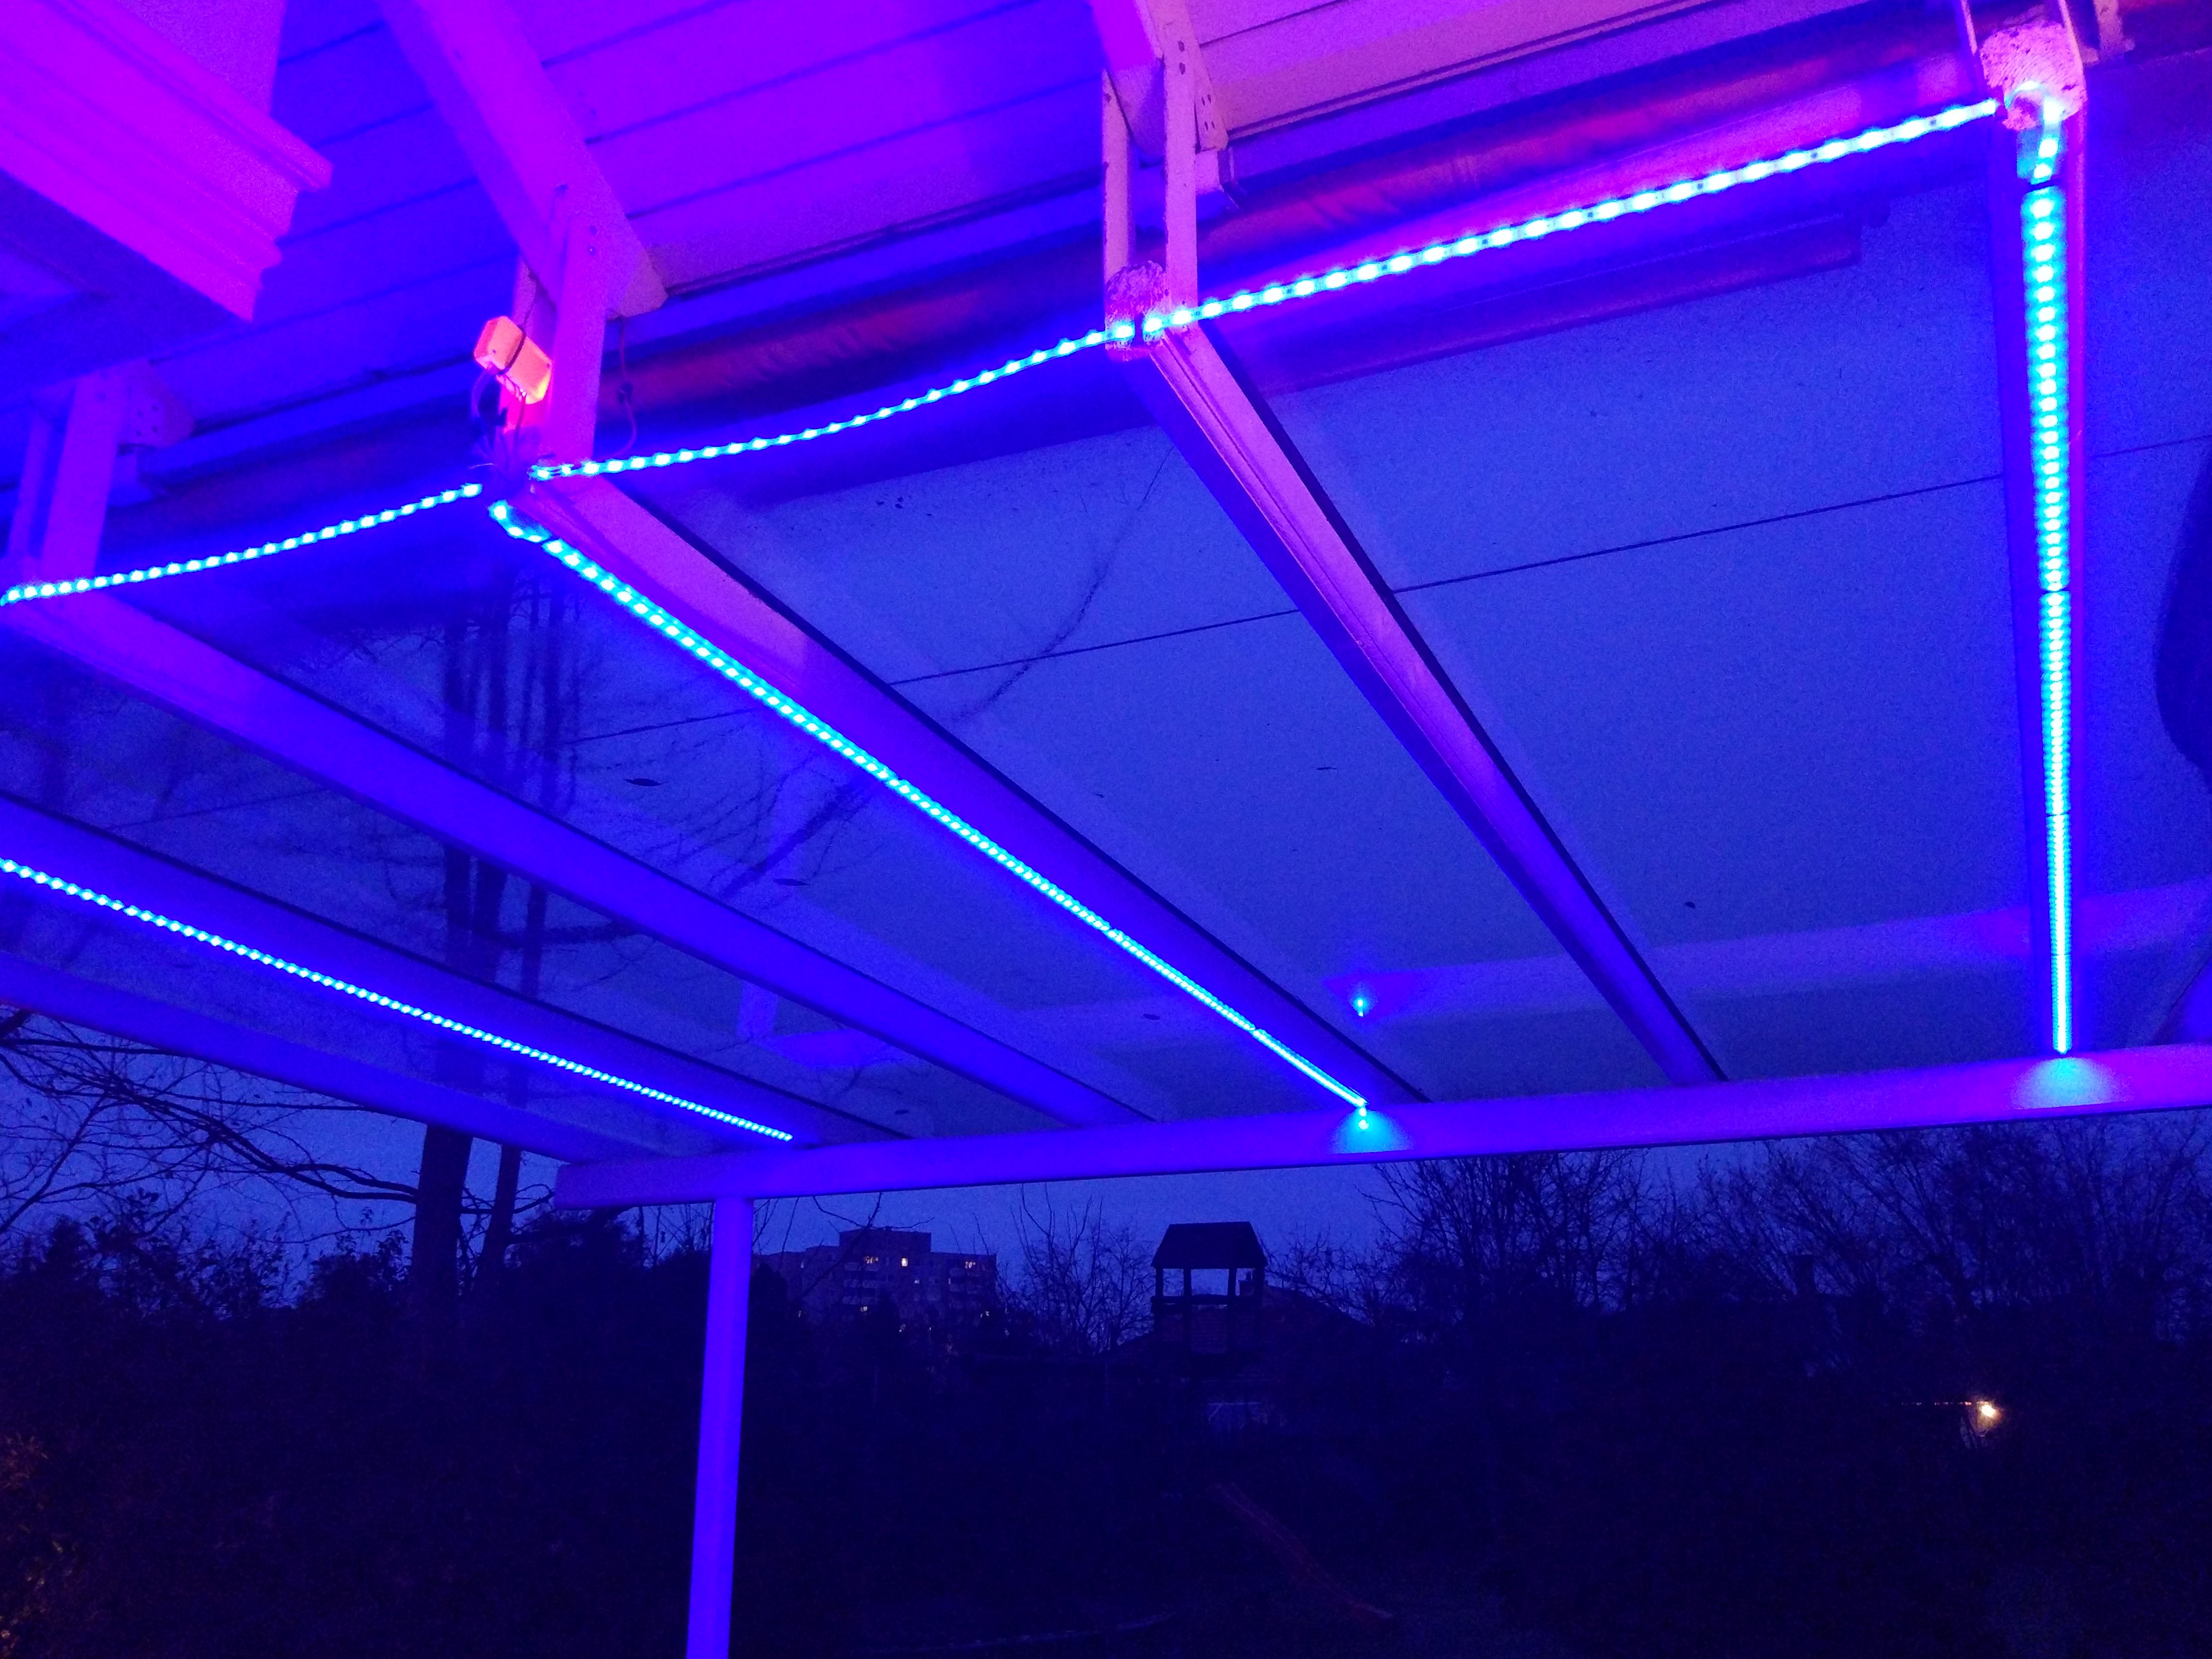
\includegraphics[height=3.8cm]{resources/alk_res/2_purpule_blue}
                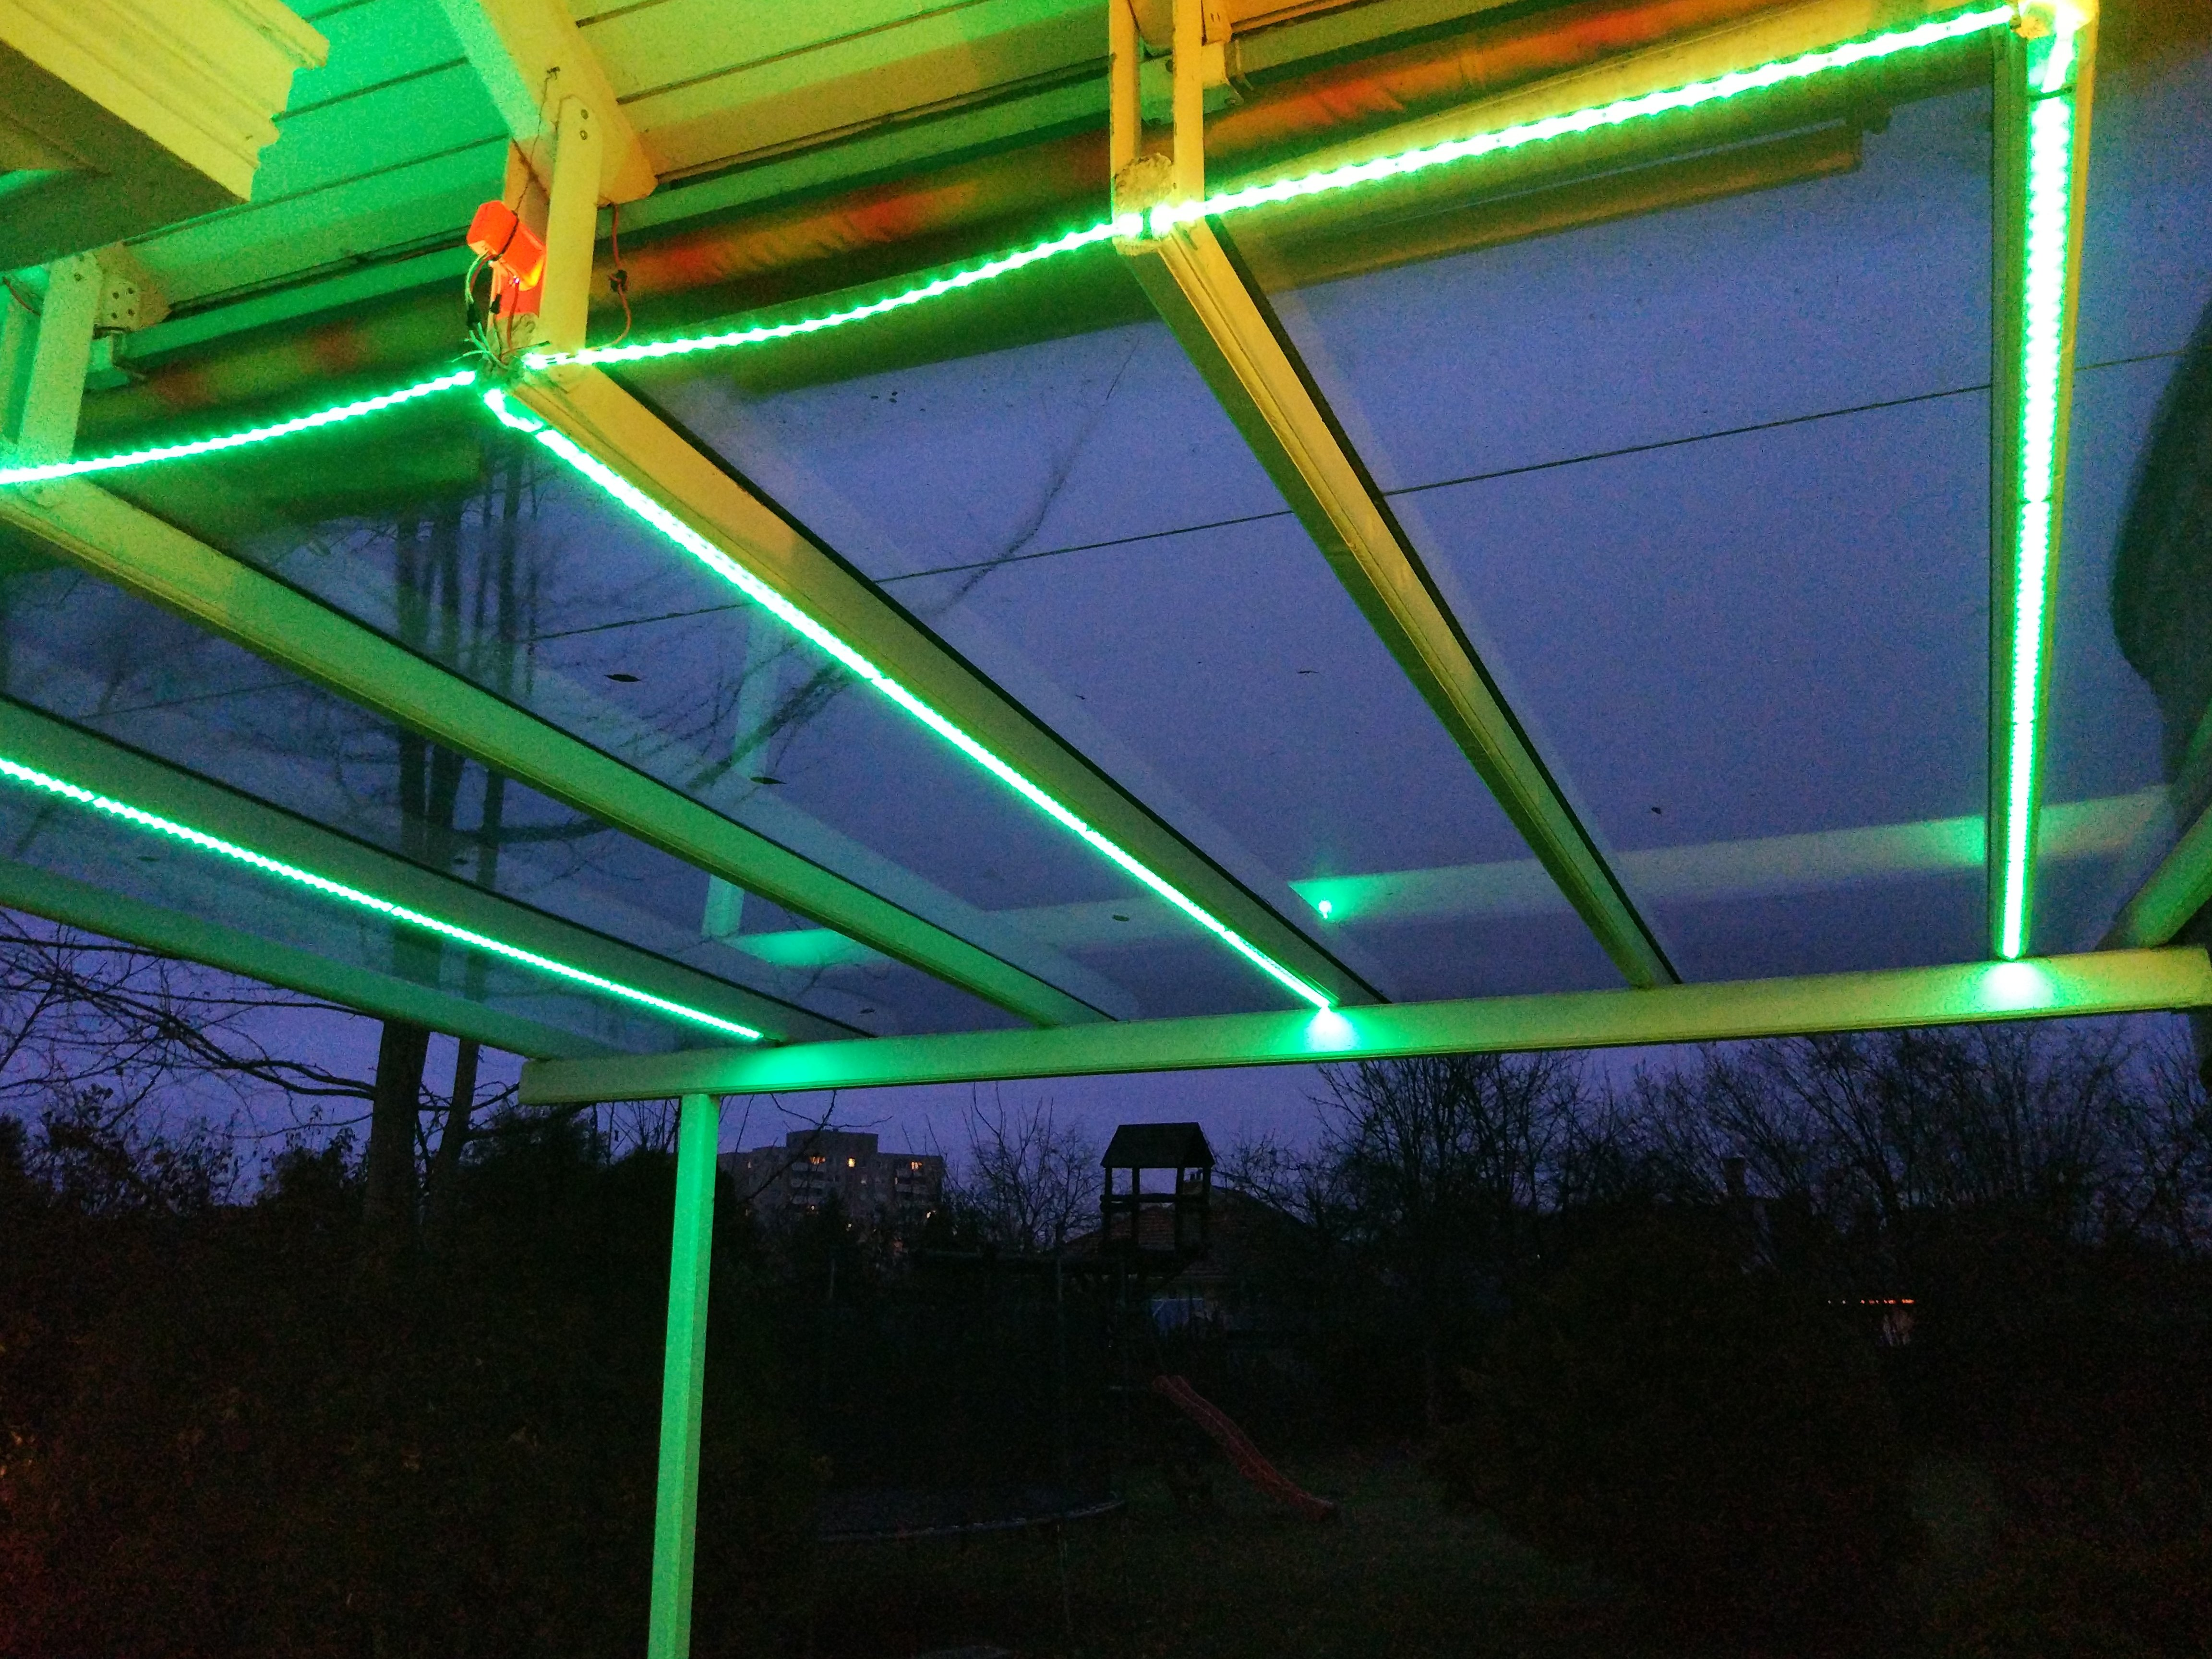
\includegraphics[height=3.8cm]{resources/alk_res/3_green}
                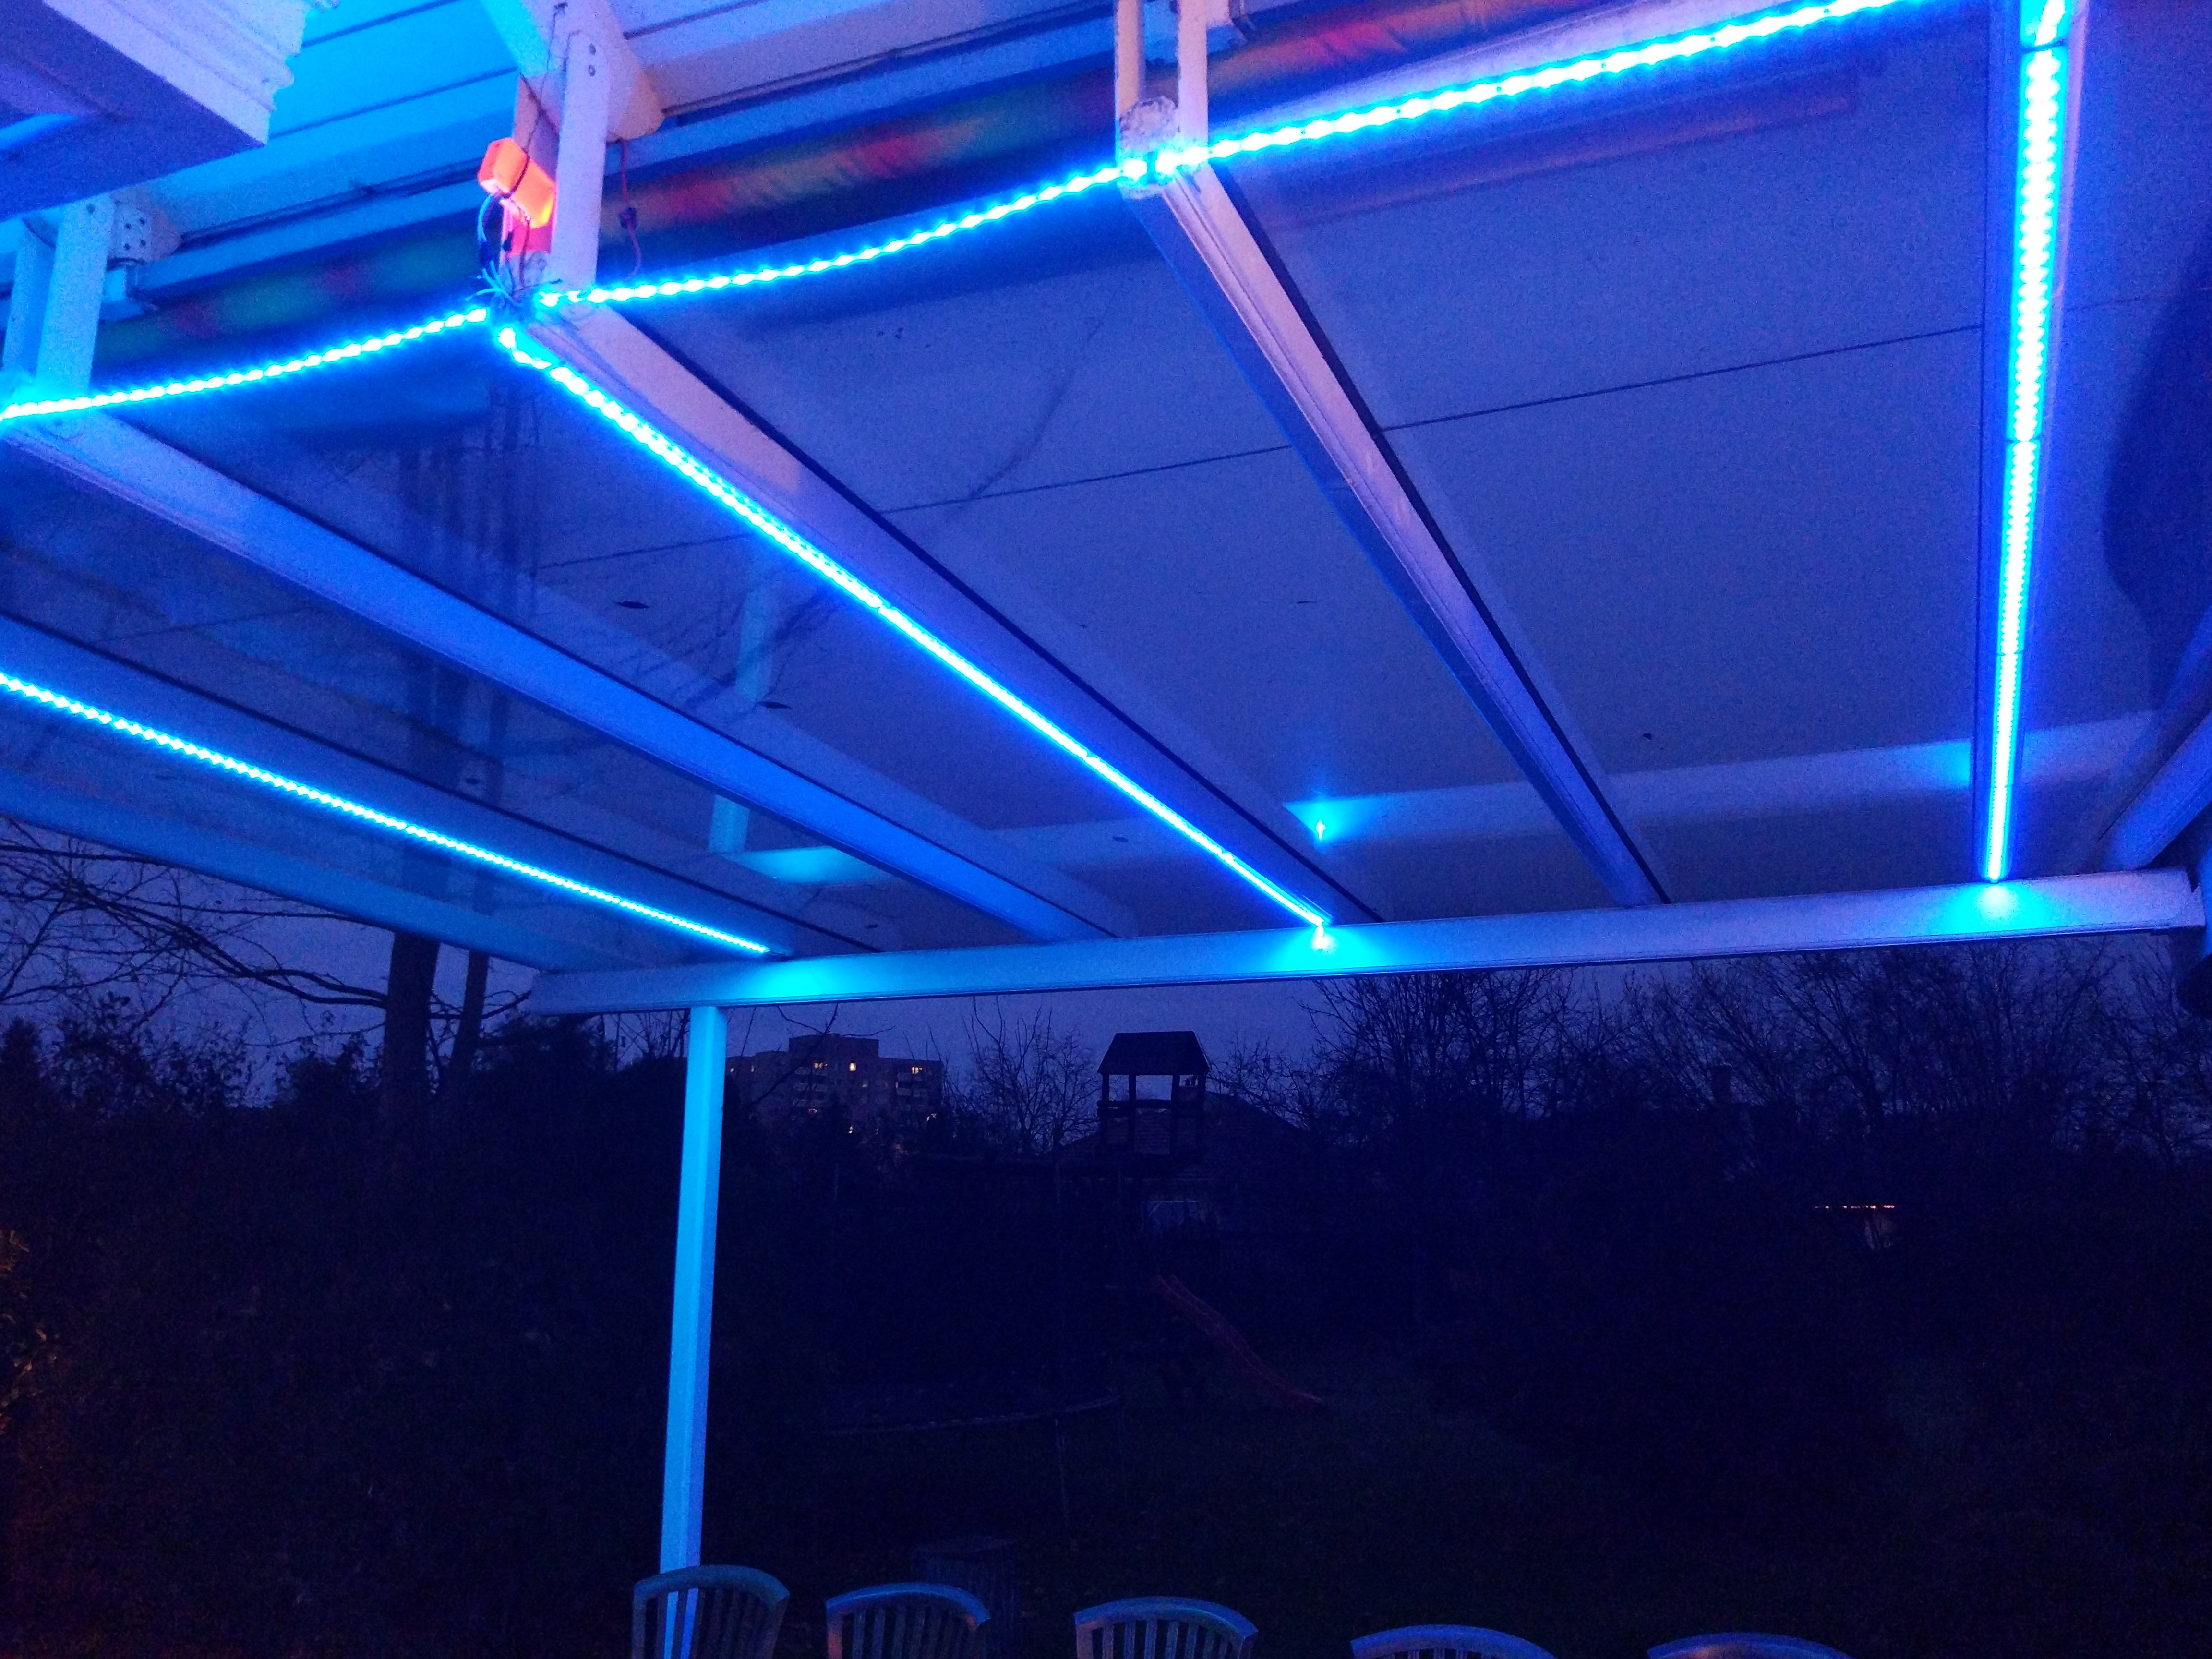
\includegraphics[height=3.8cm]{resources/alk_res/6_light_blue}
                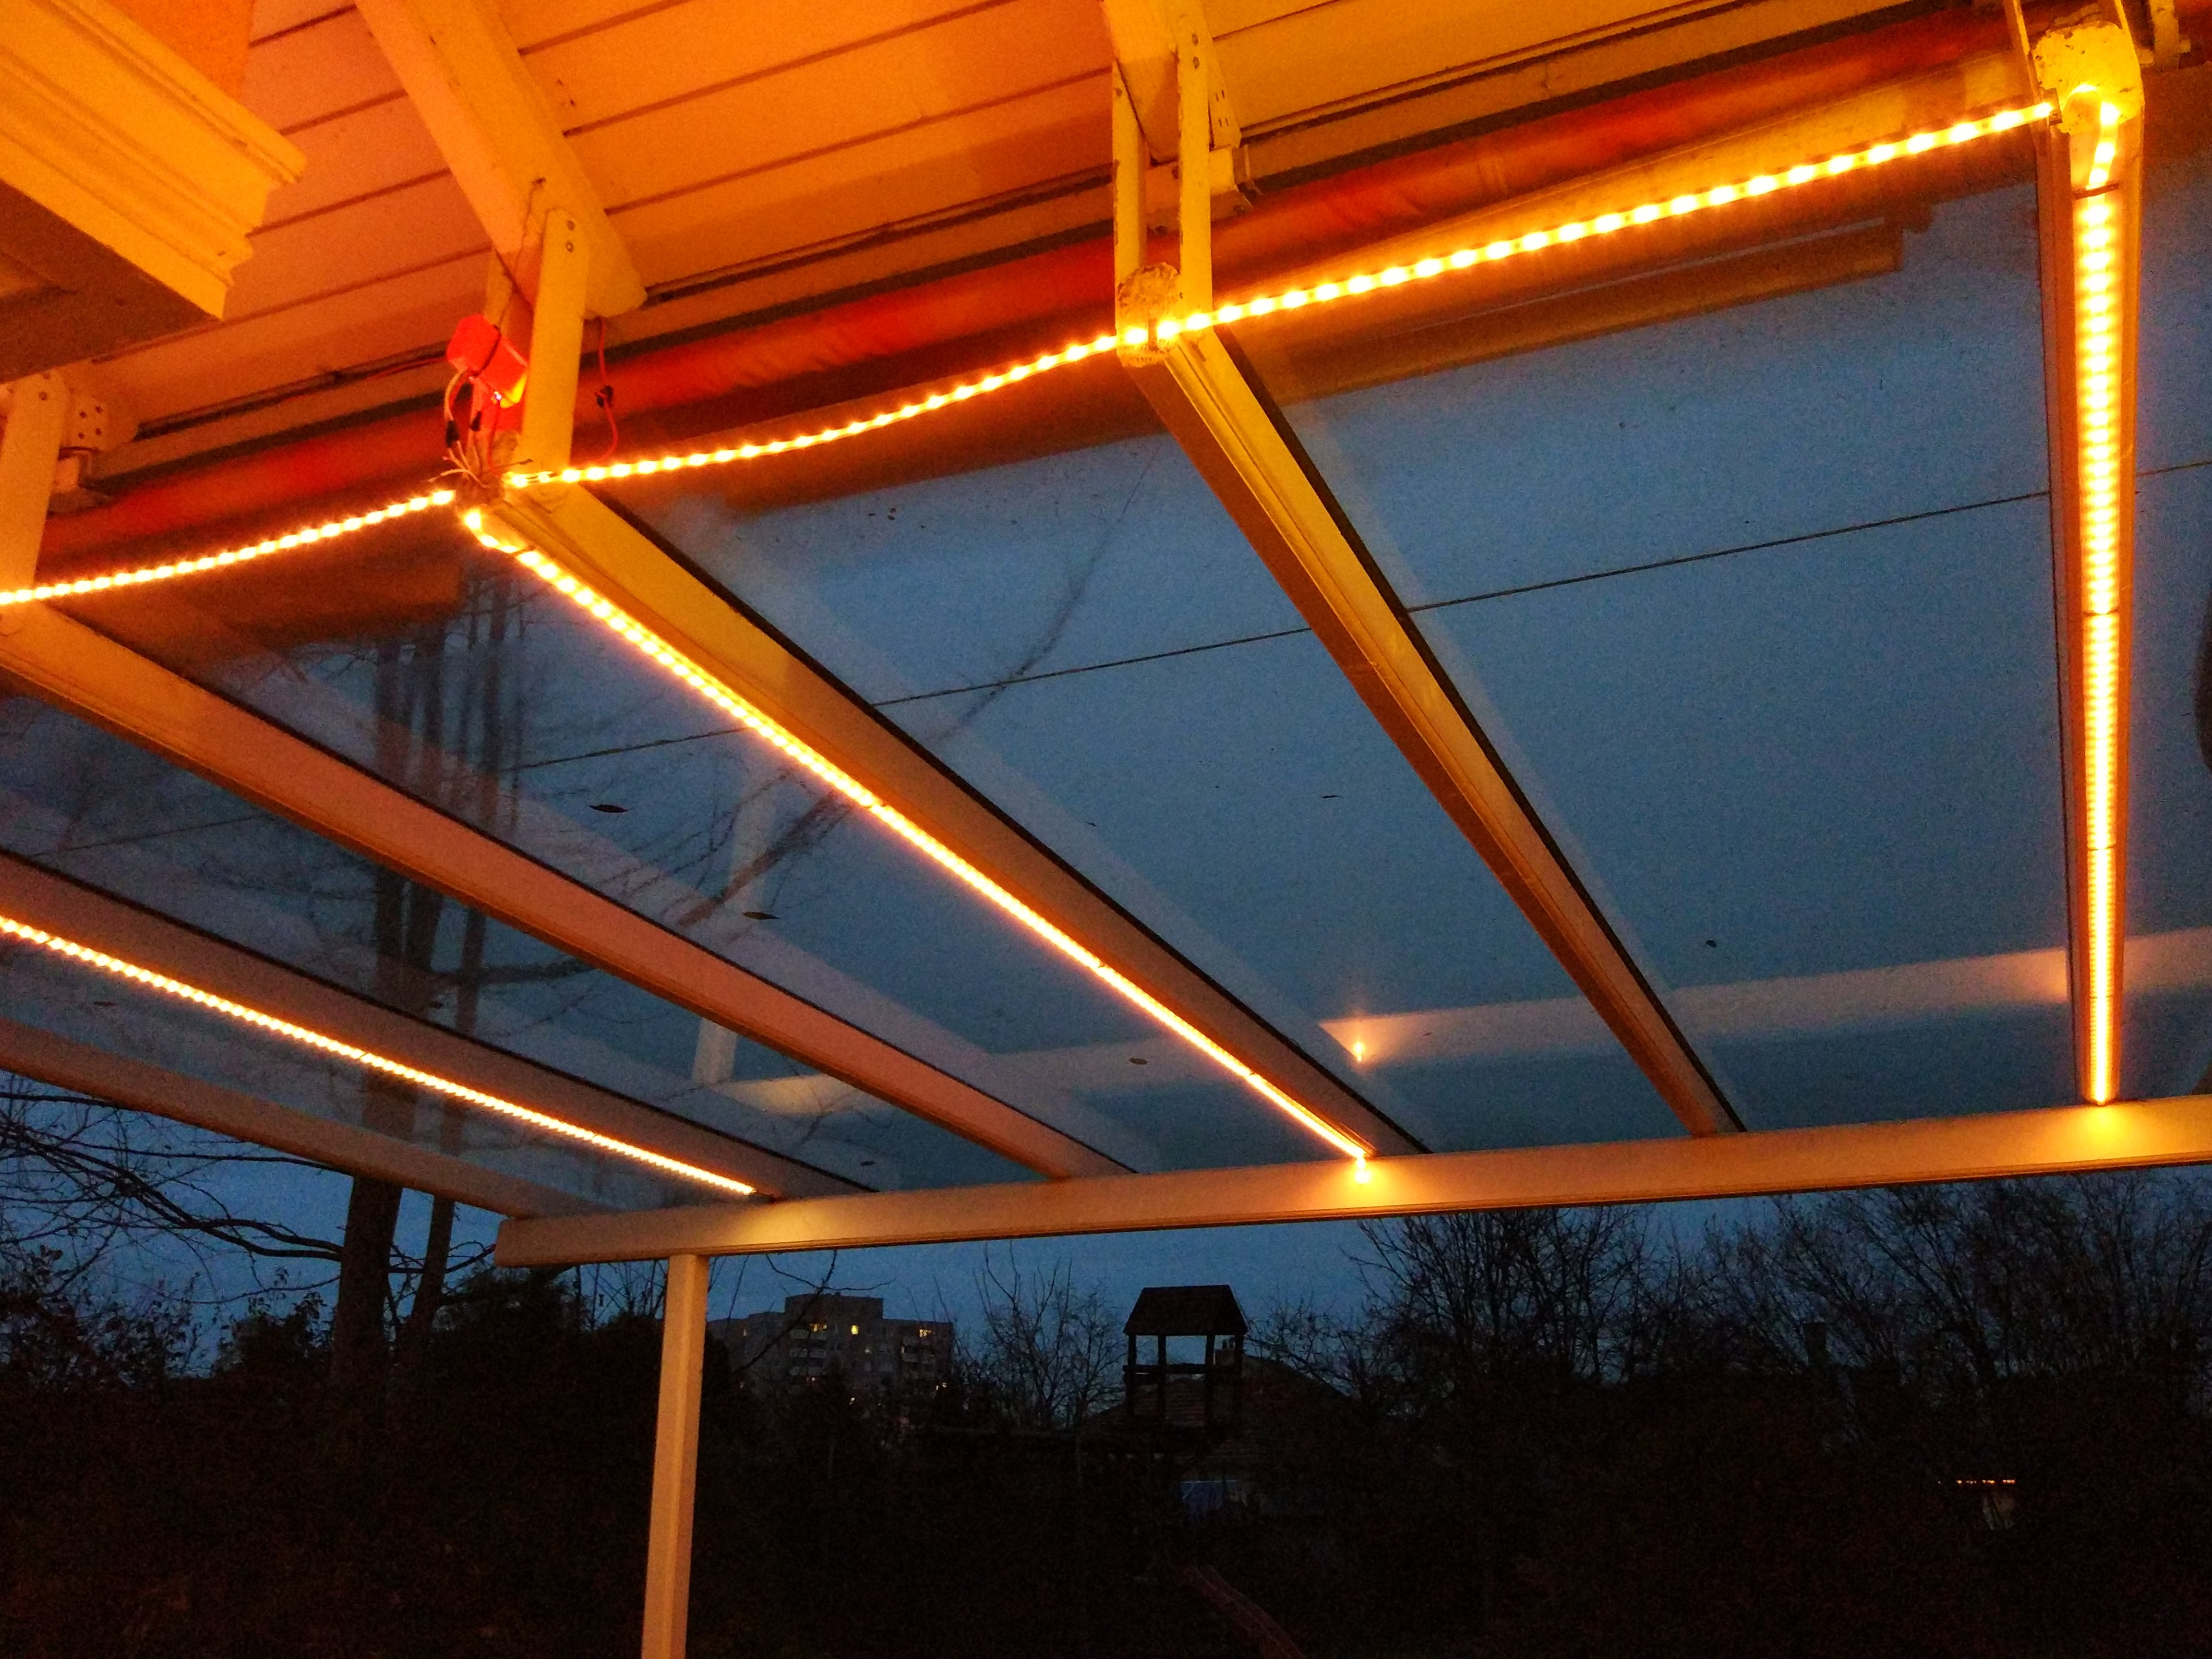
\includegraphics[height=3.8cm]{resources/alk_res/4_orange}
                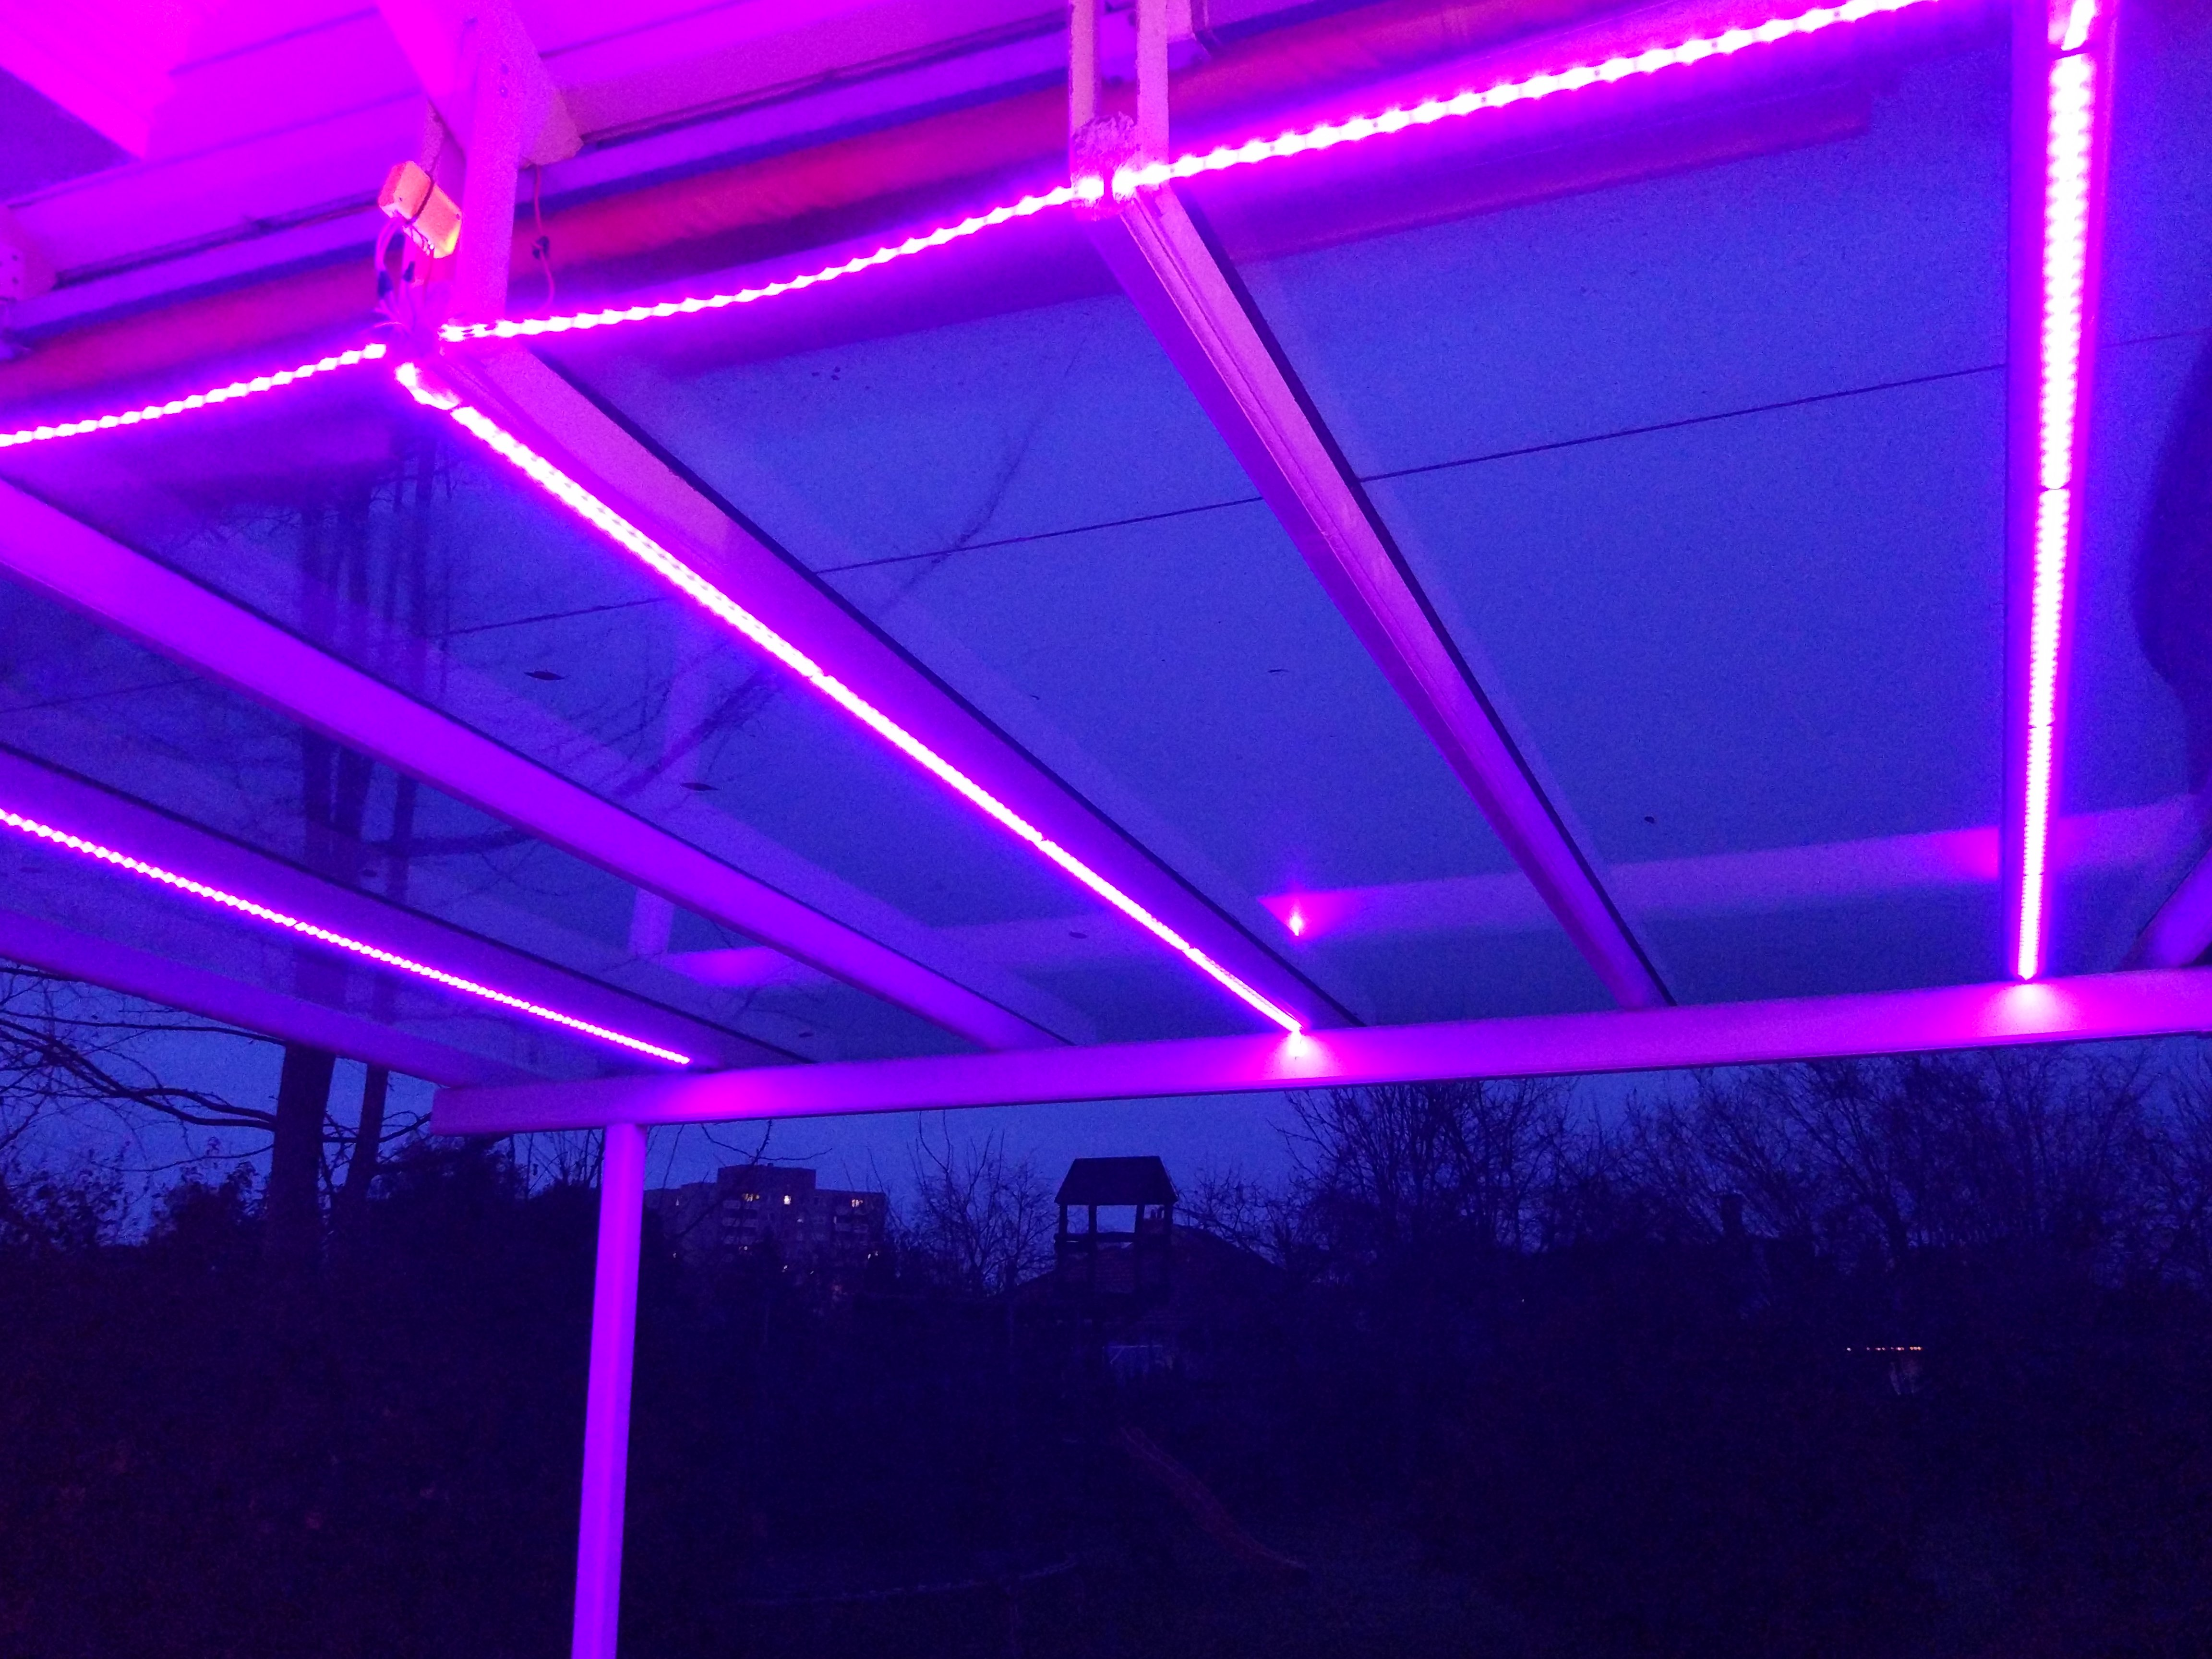
\includegraphics[height=3.8cm]{resources/alk_res/5_pink}
            \caption{Az elkészült eszköz kölönböző színeiben pompázva}
            \label{fig:pic_terasz}
        \end{figure}

        A feladat során megtanultam a Git verzió kezelő rendszer használatát, elmélyítettem mind az objektumorientált Java, illetve hardver közeli C programozói tudásom is. Átismételtem, és kibővítettem a 3D-modellezési ismereteim. Új tapasztalatokat, ismereteket szereztem a forrasztás és a 3D nyomtatás területén. 
    
    

Elegendő az elkészült utolsó eszköz költségtervét összeállítani
Szerepeljen itt még egy összegzés az elvégzett munkáról és a fejlesztési lehetőségel felsorolása
    mennyibe kerult most az 5 db prototipus nyak legyartasa, illetve mennyibe kerulne ha a legolcsobb alkatreszekbol osszevalogatva, 10 000 darabot gyartanank le
    
    
    \subsection{Fejlesztési lehetőségek}
        Mind az beágyazott rendszer, mind az elkészült Android-os alkalmazáson nagyon sok mindent tovább lehetne fejleszteni, illetve rengetek plusz funkcióval ellátni. Első lépésben a kommunikációs protokol továbbfejlesztésével kezdeném, hogy komplexebb szerkezetű adatokat, mint például új színpalettákat, lehessen küldeni a vezérlőegység számára.
        
        A beágyazott rendszer esetében fontosnak tartom egy erősebb mikrokontroller és egy mikrofon alkalmazását. Így nem kellene az Androidos alkalmazáson keresztül a zeneszámot Fourier transzformálni és 20-30 milliszekundumonként színeket küldözgetni a vezérlő egységnek, hanem saját magának számolná ki a szükséges adatokat. Ezzel jelentős mennyiségben lehetne a hálózati kommunikáció forgalmát csökkenteni és a telefon akkumlátoridejét növelni. A szoftvert fel lehetne készíteni komolyabb animációk megjelenítésére, folyamatok beütemezésére. Fejleszteni lehetne a zenére való színváltoztatást, kivilágosodást.
        
        Az Android-os applikációban biztosítani lehetne a különböző zeneszámok lejátszását. Ki lehetne bővíteni hangvezérléssel, és egy olyan nézettel, ahol ledgroup csoportoknak, de akár egysesével is, lehetne változtanti a színét. Több nyelvű felhasználói felület megalkotása sem lenne utolsó szempont, az angolul nem tudó felhasználók számára. 
        
        % Az vezélőegység további perifériák, szenzorok alkalmazásával és az Internetre való csatlakoztatásával az IoT (Internet of Things) eszközök világába is becsatlakozna\cite{a_iot}.
        
\end{document}